\documentclass{amsart}

\usepackage[T1]{fontenc}
\usepackage[utf8]{inputenc}
\usepackage[UKenglish]{babel}
\usepackage{amsmath}
\usepackage{amsthm}
\usepackage{amssymb}
\usepackage{float}
\usepackage{graphicx}
\usepackage{algorithm}
\usepackage{algorithmic}
\usepackage{todonotes}
\usepackage{enumitem}
\usepackage[misc]{ifsym}
\usepackage[foot]{amsaddr}
\usepackage[hidelinks]{hyperref}
\usepackage[style=authoryear,ibidtracker=false,uniquename=false,giveninits=true,terseinits=true,maxbibnames=5,backend=biber]{biblatex}
\renewbibmacro{in:}{}
\addbibresource{lit.bib}

\newcommand{\np}{\mathcal{NP}}
\newcommand{\parent}{\mathrm{parent}}
\newcommand{\mrca}{\mathrm{mrca}}
\newcommand{\rank}{\mathrm{rank}}
\newcommand{\nni}{\mathrm{NNI}}
\newcommand{\rnni}{\mathrm{RNNI}}
\newcommand{\rnniu}{\mathrm{RNNIu}}
\newcommand{\tbr}{\mathrm{TBR}}
\newcommand{\spr}{\mathrm{SPR}}
\newcommand{\csort}{\textsc{Caterpillar Sort}}
\newcommand{\findpath}{\textsc{FindPath}}
\newcommand{\mdtree}{\textsc{MDTree}}

\newtheorem{definition}{Definition}
\newtheorem{theorem}[definition]{Theorem}
\newtheorem{conjecture}[definition]{Conjecture}
\newtheorem{lemma}[definition]{Lemma}
\newtheorem{corollary}[definition]{Corollary}
\newtheorem{proposition}[definition]{Proposition}

\graphicspath{{figures/}}


\title[Ranked Nearest Neighbour Intarchange]{Geometry of Ranked Nearest Neighbour Interchange Space of Phylogenetic Trees}
\date{\today}
\author{Lena Collienne\textsuperscript{1}}
\email{lena.collienne@postgrad.otago.ac.nz}
\address{\textsuperscript{1}Department of Computer Science, University of Otago, New Zealand}
\author{Mareike Fischer\textsuperscript{2}}
\email{email@mareikefischer.de}
\address{\textsuperscript{2}Institute for Mathematics and Inofrmatics, University of Greifswald, Germany}
\author{David Bryant\textsuperscript{3}}
\email{david.bryant@otago.ac.nz}
\address{\textsuperscript{3}Department of Mathematics and Statistics, University of Otago, New Zealand}
\author{Alex Gavryushkin\textsuperscript{1, \Letter}}
\email{\textsuperscript{\Letter}alex@biods.org}


\begin{document}

\maketitle

\begin{abstract}

\end{abstract}

The nearest neighbour interchange ($\nni$) graph, defined on the set of phylogenetic trees with adjacency relation given by the interchange operation of two sister clades, has been known in mathematical biology literature for nearly 50 years \autocite{Robinson1971, Moore-Goodman-Barnabas1973}.
Considered with the metric given by the length of a shortest path (graph-distance), this graph becomes a metric space.
Its geometry has been extensively studied \autocite{...}.
An important property of the $\nni$ graph is that computing distance is NP-hard \autocite{...}.
As a result no algorithm exists to compute the distance in practical time \autocite{...Whidden may be}.
A consequence is that tree search and sampling algorithms pose a significant challenge even for moderately sized trees \autocite{...}.

More recent advances in computational phylogenetics introduce various classes of molecular clock models \autocite{...} and made possible computational inference of phylogenetic time-trees \autocite{...}.
However, mathematical challenges that come with this seemingly inessential change in parametrisation (genomic distance VS time distance) of trees have only recently been brought to attention \autocite{Gavryushkin2016-uu}.
\textcite{Gavryushkin2018-ol} have proposed an extension of the $\nni$ graph to the class of discrete time-trees.
The simplest such extension introduces the $\rnni$ graph on the set of ranked phylogenetic trees.
Considered with the graph-distance $\rnni$ becomes a metric space and inherits the geometric and algorithmic challenges that the $\nni$ space has been traditionally facing.
Surprisingly, most of them cannot be settled by directly translating results or applying techniques developed for $\nni$ \autocite{Gavryushkin2018-ol}.

\todo{LC: mention some results here and how they make $\rnni$ differ from $\nni$}
This distinguishes $\rnni$ from $\nni$ where this does not hold.
One further result, presented in Section~\ref{section:diameter}, directly following from the proof of Theorem~\ref{thm:caterpillar_convex}, is the diameter of $\rnni$.
Finally, we disprove the so-called Strong Split Theorem, conjectured in \autocite{Gavryushkin2018-ol}.
However, the Weak Split Theorem remains a conjecture.
Furthermore, we propose an alternative (even weaker) version of the conjecture, the Cluster Theorem (Section~\ref{section:cluster_theorem}).



In this paper, we consider the $\rnni$ space on the ranked phylogenetic trees with all taxa being of equal rank.
An example of such a tree is depicted in Figure~\ref{fig:...}.
In the terminology of \autocite{Gavryushkin2018-ol}, the space considered in this paper is the space of ranked ultrametric phylogenetic trees $\rnniu$.
We postpone accurate definitions until later in this section.

[Figure of ranked tree]

In line with the research programme proposed in \autocite{Gavryushkin2018-ol}, we investigate the geometry and algorithmic complexity of the $\rnni$ space.
Specifically, in this paper we establish the exact radius and diameter of the space, [... -- Lena, please finish this including the approximate algorithm that works exactly on small spaces (Lena: is it already in the text?)]
The question of whether there exists a polynomial algorithm for computing the $\rnni$ distance remains an open problem.

In the rest of this chapter we formally introduce non-standard definitions necessary for this paper.

A \emph{ranked phylogenetic tree} is a pair consisting of a rooted binary phylogenetic tree $T$ on the set $X = \{1, \ldots, n\}$ of \emph{taxa} for $n \in \mathbb N$, and a (total) rank function $\rank$ that maps all leaves of $T$ to $0$, all internal nodes of $T$ onto the set $\{1, \ldots, n-1\}$, and respects the partial order given by the tree.
The latter means that if $u$ and $v$ are two internal nodes of $T$ such that there exists a path from a taxon $x \in X$ to the root which first passes through $u$ and then through $v$ then $\rank(u) < \rank(v)$.
Ranked trees $(T_1, \rank_1)$ and $(T_2, \rank_2)$ are different if trees $T_1$ and $T_2$ are different or $T_1 = T_2$ and $\rank_1 \neq \rank_2$.
Since all trees in this paper are ranked trees, we will abuse the notation and drop the ranking from the notation.
We will also refer to a ranked tree simply by tree.
For a tree $T$, we will use $\rank_T$ to refer to its ranking.

Our definition of a ranked tree implies a natural notion of the edge length.:
A tree edge $(u,v)$ of $T$ has length $l$ if $|\rank_T(v) - \rank_T(u)| = l$.

Now we are ready to define the tree space which is the subject of study in this paper, the $\rnni$ graph.

The vertex set of the $\rnni$ graph is the set of all ranked trees on $n$ taxa.
We introduce two types of operation ($\rnni$ \emph{moves}) on trees (see Figure~\ref{fig:RNNI}) and say that two trees are adjacent in the $\rnni$ graph if they are connected by an operation of either type.
The first type of operation is called a \emph{rank move} and defined by swapping the ranks of two internal nodes that are not adjacent in the tree.
Formally, if $u$ and $v$ are such nodes of a tree $T$ that $|\rank_T(u) - \rank_T(v)| = 1$ and $(u, v)$ is not an edge in $T$ then the tree $R$ obtained from $T$ by only changing $\rank_R(u) = \rank_T(v)$ and $\rank_R(v) = \rank_T(u)$ is said to be obtained by a rank move.
The second type of operation is called an $\nni$ \emph{move} and defined in the usual way, that is, two trees $T$ and $R$ are said to be connected by an $\nni$ move if there exist internal edges $e$ in $T$ and $f$ in $R$ both of length one such that the trees obtained by shrinking $e$ and $f$ to internal nodes coincide.

We use the notation $d(T, R)$ throughout the paper to denote the graph distance between trees in $\rnni$, that is, $d(T, R)$ is the length of a shortest $\rnni$ path between tree $T$ and $R$.

\todo{Add a bit more space in all figures at the bottom to have at least a standard interval above he caption.}
\todo{In this figure -- rm arrows (think how to place the RNNI edges), possibly avoid using colour, and highlight where the rank move is made (hollow nodes?)}
\todo{Two of these trees are caterpillar trees.
Do you think it would be helpful to draw them as caterpillars to prepare readers for the rest of the paper?}
\begin{figure}[H]
	\centering
	\includegraphics[width=0.8\textwidth]{RNNI}
    \vspace{12pt}
	\caption{Two types of operation that define edges of the $\rnni$ graph.
    The move at the top left is a rank move while the trees in the triangle are connected by $\nni$ moves.}
	\label{fig:RNNI}
\end{figure}


\todo{LC: Explain structure of paper}


\section{Algorithms}
\label{section:algorithms}

Within this section we will at first described how we can compute exact distances between trees in the $\rnni$ graph (Section~\ref{section:alg_RNNI_graph}) by using results of \autocite{Gavryushkin2018-ol}.
Afterwards, we introduce two algorithms, namely $\findpath$ (Section~\ref{section:alg_findpath}) and $\csort$ (Section~\ref{section:alg_csort}), for computing paths between two given trees in $\rnni$.
The first one takes arbitrary trees as input while the latter one is restricted to trees with a certain tree shape.
We will use them later to prove some geometric properties of the $\rnni$ graph in section~\ref{section:geometry}.
Additionally we will present the algorithm $\mdtree$, which produces a tree that is far away from the given input tree.
What we mean by far away depends on the input tree and will be discussed after introducing this algorithm in Section~\ref{section:alg_mdtree}.

\subsection{Computing the $\rnni$ graph}
\label{section:alg_RNNI_graph}

In Section 3.3 of \autocite{Gavryushkin2018-ol} an exact algorithm for computing the $\rnni$ graph has been introduced.
We implemented this algorithm and used it for computing this graph for trees on up to seven taxa.
\todo{LC: $7$ or $8$? - I'll need to check this}
Once the graph is computed, one can get distances by using algorithms such as Floyd-Warshall \autocite{Floyd1962-ew} or Dijkstra \autocite{Dijkstra1959-ph}.
However, the large number of vertices in $\rnni$ is an obstacle when it comes to computing distances.
Since there are $\frac{n!(n-1)!}{2^{n-1}}$ vertices in the $\rnni$ graph \autocite{Gavryushkin2018-ol}, we already run out of space when we want to save all pairwise distances for trees on seven taxa.
Therefore, we compute distances between certain pairs of trees and use the symmetry of $\rnni$ to draw conclusions about the remaining distances.


\subsection{$\findpath$}
\label{section:alg_findpath}

Before introducing the algorithm we need the following definitions.
Each node $v$ of a tree defines a \emph{cluster} $C$, which is the set of taxa descending from $v$.
We then say that $v$ \emph{induces} $C$.
\emph{Trivial clusters} are clusters induced by leaves (contain just one element each) and the root of the tree (contains all taxa).
Note that the list of all non-trivial clusters of a tree, sorted according to the rank of the corresponding node, defines the tree unambiguously.
For the rest of this paper we will use the notion cluster and mean non-trivial clusters only because all trees on $n$ taxa share the trivial clusters.
We will refer to this list of clusters $n-2$ of a given tree on $n$ taxa as \emph{cluster representation} of the tree.

We are now presenting $\findpath$ (Algorithm~\ref{alg:find_path}), an algorithm for computing paths between any two given trees in $\rnni$.
Let $[C_1, \ldots, C_{n-2}]$ be the cluster representation of $R$ (the destination tree).
Then $C_i$ is induced by the node with rank $i$ for $i = 1, \ldots, n-2$.
$\findpath$ computes a path $p$ which initially consists of $T$ only and is extended stepwise.
In order to do this, the clusters $C_1, \ldots, C_{n-2}$ of $R$ are considered in that order.
Let $T'$ be the last tree of $p$ when arriving at cluster $C_k$.
We assume that the clusters $C_1, \ldots, C_{k-1}$ are induced by nodes of rank $1, \ldots, k-1$ in $T'$, respectively.
In the first step it is $T' = T$ and $C_k = C_1$.
The aim is now to find a sequence of $\rnni$ moves, starting at $T'$, that do not change the clusters $C_1, \ldots, C_{k-1}$, but result in a tree containing clusters $C_1, \ldots, C_{k}$.
Therefore, we need to find the smallest cluster containing all elements of $C_k$ in $T'$.
This node is denoted by $\mrca_{T'}(C_k)$ (short for \emph{most recent common ancestor}).
The rank of $\mrca_{T'}(C_k)$ in $T'$ is higher than the rank of the node inducing $C_k$ in $R$, because $C_1, \ldots, C_{k-1}$ are already present in $T'$ and we assume that $C_k$ is not.
Now perform an $\rnni$ move that decreases the rank of $\mrca_{T'}(C_k)$.
With Lemma~\ref{lemma:mrca_move} we know that such an $\rnni$ move always exists if long as $T'$ does not induce the cluster $C_k$.
So we can perform such moves until a tree $T''$ with $\mrca_{T''}(C_k)$ is reached that contains a node inducing $C_k$ that has the same rank $k$ in $T''$ as in $R$.
Appending all trees on this path from $T'$ to $T''$ and repeating this procedure for all clusters of $R$ results in a path $p$ from $T$ to $R$.

\begin{algorithm}[H]
\caption{$\findpath$($T,R$)}
\label{alg:find_path}
\begin{algorithmic}[1]
	\STATE $T' := T$
	\STATE $p := [T']$
	\FOR {$i = 1, \dots, n-2$}
		\STATE Let $C_i$ be the cluster induced by the node with rank $i$ in $R$ \label{alg:find_path:line:cluster}
		\WHILE {$\rank_{T'}(\mrca_{T'}(C_i))>i$}
			\STATE Update $T'$: Decrease $\rank_{T'}(\mrca_{T'}(C_i))$ by an $\rnni$ move \label{alg:findpath:line:move_set_down}
			\STATE $p = p+T'$
		\ENDWHILE
	\ENDFOR
	\RETURN $p$
\end{algorithmic}
\end{algorithm}

The following lemma shows that $\findpath$ gives a path between the two input trees, indeed, by proving that there is always an $\rnni$ move possible as described in Line~\ref{alg:findpath:line:move_set_down} of Algorithm~\ref{alg:find_path}.

\begin{lemma}
    Let $T$ and $R = [C_1, \ldots, C_{n-2}]$ be two trees and $p:= \findpath (T,R)$ a path from $T$ to $R$.
    Let $T' \neq T,R$ be a tree on $p$ such that $C_1, \ldots, C_{k-1}$ are induced by internal nodes of $T'$, but $C_k$ is not.
    Then there is always exactly one $\rnni$ move on $T'$ that results in a tree $T''$ such that $\mrca_{T''}(C_i) < \mrca_{T'}(C_i)$.
    \label{lemma:mrca_move}
\end{lemma}

\begin{proof}


    Let $T, R$ and $T'$ be trees as defined in the lemma and $[C_1, \ldots, C_{n-2}]$ the cluster representation of $R$.
    We want to prove that there is exactly one $\rnni$ move on $T'$ that results in a tree $T''$ where $\mrca_{T''}(C_k) < \mrca_{T'}(C_k)$.
    Notice, that the only $\rnni$ move on $T$ that could decrease the rank of $\mrca_{T'}(C_k)$ are $\nni$ movs on the edge between $\mrca_{T'}(C_k)$ and its child (if this edge has length one), or a rank move between $\mrca_{T'}(C_k)$ and the node with rank one less.
    Therefore, we will now distinguish these two cases:
    Either there is an edge $(v,w)$ between nodes $v = \mrca_{T'}(C_k)$ and $w$ with rank $rank_{T'}(w) = rank_{T'}(v) - 1$, or there is no such edge.

    In the latter case the only $\rnni$ move that could increase the rank of $v$ is a rank move swapping the ranks of $v$ and $w$.

    If there is an edge $(v,w)$ in $T'$ there are two $\nni$ moves possible on this edge.
    We are now going to explain why only one of these two $\nni$ moves changes the rank of this most recent common ancestor.
    By definition we know that $C_1, \ldots, C_{k-1}$ are induced by the nodes of rank $1, \ldots, k-1$, respectively, in $T'$ already.
    It is important to notice that $C_k$ either is the disjoint union $C_k = C_i \dot\cup C_j$ for $i,j < k$ or $C_k = C_i \dot\cup \{x\}$ for a taxon $x \in X \setminus (C_1 \cup \ldots \cup C_{k-1})$.

    Le us at first assume that $C_k = C_i \dot\cup C_j$ for some $i,j < k$.
    The tree $T'$ looks like the tree depicted in the left of Figure~\ref{fig:mrca_move} where $T_w^1$ and $T_w^2$ are the two subtrees rooted in the children of $w$ and $T_v$ is the subtree whose root is child of $v$ and does not include $w$.
    Since we know that all clusters $C_1,\ ldots, C_{k-1}$ are induced by some nodes in $T'$, each of these clusters must be a subset of the taxon set of one of the three subtrees $T_w^1,T_w^2$, or $T_v$.
    In particular, there can't be elements of the same cluster $C_m$ in more than one of these subtrees.
    This and the fact that $v = \mrca_{T'}(C_i \dot\cup C_j)$ yields that either $C_i$ or $C_j$ is subset of the taxon set of $T_v$ and the other cluster is subset of the taxon set of either $T_w^1$ or $T_w^2$.

    Without loss of generality we assume that $C_i$ is included in $T_v$.
    Otherwise, change the indices $i$ and $j$.
    Then $C_i$ is a subset of the taxon set of either $T_w^1$ or $T_w^2$.
    Therefore, just one of the two $\nni$ moves on $(v,w)$, as depicted in Figure~\ref{fig:mrca_move}, moves the most recent common ancestor of $C_k = C_i \dot \cup C_j$ down.

    Now we consider the case that $C_k = C_i \dot\cup \{x\}$ for a taxon $x \in X \setminus (C_1 \cup \ldots \cup C_{k-1})$.
    For the same reason as above, $C_i$ is in subset of the taxon set of one of the subtrees $T_w^1, T_w^2$ or $T_v$ of $\hat T$ as depicted in Figure~\ref{fig:mrca_move}.
    Similarly $x$ is taxon of one of these three subtrees in a way that either $C_i$ or $x$ is included in $T_v$, because $v = \mrca_{T'}(C_i \dot \cup \{x\})$.
    So there is just one of the two subtrees $T_w^1$ and $T_w^2$ that neither includes $C_j$ nor $x$.
    As in the previous case, just one of the two $\nni$ moves on $(v,w)$ as illustrated in Figure~\ref{fig:mrca_move} decreases the rank of $\mrca_{T'}(C_i \dot \cup \{x\})$.

    We can conclude that in any case there is exactly one $\rnni$ move possible on $T'$ that decreases the rank of $\mrca_{T'}(C_k)$ in Line~\ref{alg:findpath:line:move_set_down} of Algorithm~\ref{alg:find_path}.

    \begin{figure}[H]
    	\centering
    	\includegraphics[width=0.5\textwidth]{mrca_move}
        \vspace{12pt}
        \caption{Two $\nni$ moves that are possible on the edge $(v,w)$ of the tree $T'$.
        They result in the trees on the right as described in the proof of Lemma~\ref{lemma:mrca_move}.}
    	\label{fig:mrca_move}
    \end{figure}

\end{proof}

With Lemma~\ref{lemma:mrca_move} we can conclude that $\findpath$ is a deterministic algorithm.
Its running time is quadratic in the number of taxa.
Since it computes a path between two arbitrary trees in $\rnni$, we can use the length of such a path as approximation for the distance between the trees.
A natural question is how well this estimates the actual distance in $\rnni$.
To answer this question for small trees, we implemented $\findpath$.
\todo{LC: github - link}
For computing the actual $\rnni$ distances we used the the algorithm for computing the $\rnni$ graph as described in Section~\ref{section:alg_RNNI_graph}.
\todo{LC: How do we compare the distances?}



\subsection{$\csort$}
\label{section:alg_csort}


For introducing an algorithm to compute paths between caterpillar trees, we need further notations.
In this section we aim to investigate properties of paths between \emph{caterpillar trees} where each internal node has at least one child that is a leaf.
A path $p$ between two caterpillar trees $T$ and $R$ that only consists of caterpillar trees is called \emph{caterpillar path}.
If $p$ is shortest among all caterpillar paths between these trees we call it \emph{shortest caterpillar path}, and the length of $p$ will be denoted by $d_c(T,R)$ and called \emph{caterpillar distance}.

Let us now introduce a representation of caterpillar trees as lists of taxa.
This representation is basically a simplification of the cluster representation for caterpillar trees and works as follows.
For a caterpillar tree with cluster representation $T = [C_1, \ldots, C_{n-2}]$ it is $C_i \subset C_{i+1}$ with $|C_i| = |C_{i+1}|$ for all $i = 1, \ldots, n-3$.
Therefore, the list of taxa $L_T = [x_1, x_2, \ldots, x_n]$ with $x_1<x_2$ uniquely represents the caterpillar tree $T = [C_1, \ldots, C_{n-2}]$ with $C_i = \{x_1, \ldots, x_{i+1}\}$.
In this list representing a caterpillar tree the taxa are ordered non-decreasing, according to the ranks of their parents.
Note that the only two elements in such a list that have parents of equal rank are the first two elements $x_1$ and $x_2$.
That is why we order them in the list such that $x_1 < x_2$ to make the list representation of caterpillar trees unique.
We will call a pair of two taxa that share their parent \emph{cherry}.
We will use this list representation to show how one can adapt the classical \emph{Bubble Sort} algorithm \autocite{Knuth1997-pi} to compute caterpillar paths.

We are now going to explain what kind of $\rnni$ moves are possible between caterpillar trees and see how such a move changes the list representation of a tree.
At first it is important to realise that the only possible $\rnni$ moves between caterpillar trees are $\nni$ moves, since there is no pair of internal nodes with rank difference one that is not connected by an edge.
$\nni$ moves between caterpillar trees correspond to swaps of two neighboured elements in the list representation.
The only exception of this are $\nni$ moves on the lowest internal edge, that is the edge connecting the internal nodes of rank one and two.
There are two $\nni$ moves possible on this edge that result in caterpillar trees, while there is for every other edge only one $\nni$ move that results in a caterpillar tree.
Corresponding to the $\nni$ moves on the lowest internal edge are exchanges of either the first or the second element with the third element in the list representation.

By using this knowledge we can compute shortest caterpillar paths by modifying Bubble Sort as described in the following.
We call this algorithm $\csort$ (Algorithm~\ref{alg:csort}).

Let $T$ and $R$ be the input trees for $\csort$.
We assume that they are given in their list representation $L_T$ and $L_R$ as described above and want to compute a path from $L_T$ to $L_R$.
This path $p$ is built stepwise by adding a new list to the end of $p$.
We call the last element of $p$ at any step $L_{T'}$, representing a tree $T'$ and when we say we update $L_{T'}$, we modify this list and append the new version of $L_{T'}$ to $p$.

As in the Bubble Sort algorithm, we go through the list $L_{T'}$ and swap two elements if they appear in different orders in $L_{T'}$ and $L_R$.
Each swap of elements is an update of $T'$ and extends the path $p$ by one element.
We compare pairs of list elements from the start of the list until its end, and repeat this until the whole list is sorted, just as in classical Bubble Sort.
Our algorithm $\csort$ only differs from Bubble Sort when considering the first three elements of the list.
As we discussed above, both the first and second element of $L_{T'}$ can exchange with its third element.
Therefore, we need to consider these moves separately to all other moves.
Most importantly, we need to make sure that these moves are performed in a way that leads to a shortest caterpillar path.
We can guarantee this if the moves are done as described in the following.
Let $x_1, x_2$ and $x_3$ be the first three elements of $L_{T'}$, in this order.
If $x_1$ ($x_2$) is the last element of those three in $L_R$, we update $L_{T'}$ by swapping $x_1$ ($x_2$) and $x_3$.
By doing this we make sure that there will be no point on $p$ where $x_1$ and $x_2$ swap positions, which would cause an additional $\nni$ move that can be avoided if we perform the moves as described.

Because all moves between caterpillar trees are $\nni$ moves, all pairs of taxa that are not in the same order in $L_T$ and $L_R$ need to swap at some point on any path between $L_T$ and $L_R$.
And since only elements that are direct neighbours in a sequence are allowed to swap, with the only exception being the first three elements, the path computed by $\csort$ is a shortest caterpillar path.

\begin{algorithm}[H]
\caption{$\csort$($T,R$)}
\label{alg:csort}
\begin{algorithmic}[1]
    \STATE $T':= T$, $p := [T']$
    \STATE $L_{T'}:=$ list representation of $T'$, $L_R:=$ list representation of $R$
	% \STATE $L_{\hat T} :=$ list representation of $\hat T$, $L_R :=$ list representation of $R$
    \FOR {$i=1,\ldots,n-2$} \label{alg:csort:line:loop}
        \STATE $j = 0$ \COMMENT{Special case: cherry}
        \IF {$L_{T'}[0]$ is last element of $L_{T'}[0],L_{T'}[1],L_{T'}[2]$ in $L_R$}
            \STATE Update $T'$: swap $L_{T'}[0]$ and $L_{T'}[2]$
        \ELSIF {$L_{T'}[1]$ is last element of $L_{T'}[0],L_{T'}[1],L_{T'}[2]$ in $L_R$}
            \STATE Update $\hat T$: swap $L_{T'}[1]$ and $L_{T'}[2]$
        \ENDIF
        \STATE $j = 2$
	    % \IF {$L_R^{-1}[L_{\hat T}[j]] > L_R^{-1}[L_{\hat T}[j+1]]$}
        \WHILE {order of $L_{T'}[j]$ and $L_{T'}[j+1]$ different in $R$}
			\STATE Update $T'$: Swap $L_{T'}[j]$ and $L_{T'}[j+1]$
			\STATE $p = p+T', j = j + 1$
		\ENDWHILE
    \ENDFOR
	\RETURN $p$
\end{algorithmic}
\end{algorithm}

The running time of $\csort$ is the same as for Bubble Sort, that is quadratic in $n$.
Within Section~\ref{section:caterpillar_convex} we will use $\csort$ for some proofs.
Therefore it is important to notice that at the end of each loop $i$ starting in Line~\ref{alg:csort:line:loop} of Algorithm~\ref{alg:csort}, the last $i$ elements of $L_{T'}$ are the same as the ones in $L_R$.
This is a well known property of Bubble Sort that $\csort$ inherits from it.


\subsection{$\mdtree$}
\label{section:alg_mdtree}

The algorithm we are going to introduce here will be important for finding the radius of the $\rnni$ graph.
In Section~\ref{section:diameter} we will prove that it computes a tree with maximum distance from a given caterpillar tree (Lemma~\ref{lemma:max_dist_caterpillar}), which implies that the radius of $\rnni$ equals its diameter (Corollary~\ref{corollary:radius}).
Therefore, it is called $\mdtree$ (Maximum Distance Tree).

$\mdtree$ works as follows for an input tree $T$:
At first, all taxa of $T$ are sorted in a list $L$ such that the ranks of their parents are non-decreasing.
This representation is somehow similar to the list representation of caterpillar trees, but it is ambiguous since we do not specify in which order taxa appear in the list that share their parent.
If the input is a caterpillar tree, it follows that $L[0]$ and $L[1]$ are the cherry taxa of $T$, in an arbitrary order, and the parent of taxon $L[i]$ has rank $i$ in $T$ for all $i = 2, \ldots, n-1$.
$\mdtree$ builds the output tree $R$ as follows:
Initially, $R$ only consists of a cherry with taxa $L[0]$ and $L[1]$ such that the parent of these taxa has rank $n-1$.
All following taxa in $L$ are added to $R$ sequentially, according to their order in $L$, by creating a new internal node at one of the existing branches in $R$ such that this new node has rank one less than the previously lowest internal node in $R$.

Algorithm~\ref{alg:max_dist_tree} provides pseudocode for this algorithm.
We will see in Section~\ref{section:diameter} that it computes trees with maximum distance form any given caterpillar tree.
But if the given tree is an arbitrary tree, the output tree might not have maximum distance to the input tree.

\todo{LC: Shall we give an example where the distance is not max or simulate trees and compute histogram of distances approximated by $\findpath$?}

\begin{algorithm}[H]
\caption{$\mdtree(T)$}
\label{alg:max_dist_tree}
\begin{algorithmic}[1]
	\STATE $R$ only contains cherry taxa $a, b$ of $T$ and has internal node with rank $n-1$
    \STATE In list $L$ all taxa $\{1,\ldots,n\}\setminus\{a,b\}$ are ordered such that the ranks of their parents in $T$ do not decrease \label{alg:mdtree_lineL}
	\FOR {taxon $a$ in $L$}
		\STATE Add an internal node as parent of $a$ on an edge in $R$ such that the new internal node has rank one less than the previously lowest internal node \label{alg:mdtree_lineAddTaxon}
	\ENDFOR
	\RETURN $R$
\end{algorithmic}
\end{algorithm}

An important property of $\mdtree$, which we will use later on in Section~\ref{section:diameter}, is the fact that this algorithm is non-deterministic.
Because the list computed in Line~\ref{alg:mdtree_lineL} the and the attachment edge of the new taxon in the tree in Line~\ref{alg:mdtree_lineAddTaxon} are not uniquely determined, the output tree $R$ of $\mdtree$ is not unique.



\section{Geometry of $\rnni$}
\label{section:geometry}

In this section we analyse shortest paths in $\rnni$.
Therefore, we will use the algorithms introduced in the previous section.
They enable us to prove that there is always a shortest path between two caterpillar trees that only consists of caterpillar trees (Theorem~\ref{thm:caterpillar_convex}) in Section~\ref{section:caterpillar_convex}.
In other words, the set of caterpillar trees is \emph{convex} in $\rnni$.
In Section~\ref{section:diameter} we will investigate diameter and radius of the $\rnni$ graph.
Interestingly, the \emph{diameter}, that is the maximum distance $\Delta(\rnni) = \max \{d(T, R) \mid T, R \in \rnni\}$ between any two trees in the graph, of $\rnni$ equals its \emph{radius} $rad(\rnni) =  \min\limits_T \max\limits_R d(T,R)$ in $\rnni$.
After proving this, we are going to consider the so-called Split Theorem, which was raised in \autocite{Gavryushkin2018-ol}.
We will give a counterexample to disprove their version of the Split Theorem and claim an alternative version.

Before we get into the details of these geometric properties of $\rnni$, we need to prove some statements that will be used a few times within this geometry section.

\begin{lemma}
    It is $\Delta(\rnni) \leq \frac{(n-1)(n-2)}{2}$ for $n \geq 3$.
    \label{lemma:diameter_bound}
\end{lemma}

\begin{proof}
Since the diameter is bounded from above by the maximum length of a path computed by $\findpath$, it is enough to find this maximum.
The worst-case execution of $\findpath$ would require each of the $n-2$ clusters $C_i$, considered in Line~\ref{alg:find_path:line:cluster} of Algorithm~\ref{alg:find_path}, to be moved by $n-1-i$ $\rnni$ operations in $T'$.
This can happen if each cluster $C_i$ has the root as $\mrca_{T'}(C_i)$.
Then the rank of this most recent common ancestor must be changed from $n-1$ to $i$, which requires $n-1-i$ operations, according to Lemma~\ref{lemma:mrca_move}.
Hence, the maximum length of such a path is bounded by $\sum\limits_{i = 1}^{n-2} i = \frac{(n-2)(n-1)}{2}$.
\end{proof}

The following lemma relates distances between trees on $n$ and $n+1$ taxa and is an important tool for inductive arguments.
We use the notion $\parent_T(x)$ to refer to the node adjacent to taxon $x$ in tree $T$.
$T{\big|}_n$ denotes the restriction of tree $T$ to the set of taxa $\{1, \ldots, n\}$.
In particular if $T$ is a tree on taxa $1, \ldots, n+1$ the tree $T{\big|}_n$ is obtained by deleting taxon $n+1$ and suppressing the thereby created node of degree two.

\begin{lemma}
Let $T$ and $R$ be two trees on taxa $\{1, \ldots, n+1\}$.
Then $d(T{\big|}_n, R{\big|}_n) \leq d(T,R) - \delta$, where $\delta = |\rank_T(\parent_T(n+1)) - \rank_R(\parent_R(n+1))|$.
\label{lemma:distance_delete_taxon}
\end{lemma}

\begin{proof}
Let $T$ and $R$ be trees as described in the lemma.
First observe that the rank of the internal node $\parent_T(n+1)$ can only be changed by performing a rank move that involves $\parent_T(n+1)$ or an $\nni$ move on an edge adjacent to $\parent_T(n+1)$.
Second observe that any $\rnni$ move can change the rank of $\parent_T(n+1)$ by at most one.
So we can follow that an $\rnni$ on $T$ move can decrease the rank of $\parent_T(n+1)$ by at most one.

Let $p$ be a shortest path from $T$ to $R$ and $p{\big|}_n$ the path resulting from deleting taxon $n+1$ from all trees on $p$.
Then $p{\big|}_n$ is a path from $T{\big|}_n$ to $R{\big|}_n$.
The reason for this is that the only moves that are deleted from $p$ to receive $p{\big|}_n$ are those involving the parent of taxon $n+1$.
All other moves stay the same and can be performed equally on a path from $T{\big|}_n$ to $R{\big|}_n$ as on a path from $T$ to $R$, because the relations of all other internal nodes are the same between both pairs of trees.
Recall that $\delta$ is the difference in ranks between the parents of taxon $n+1$ in $T$ and $R$.
With the knowledge that an $\rnni$ move on $T$ can change the rank of $\parent_T(n+1)$ by at most one, we can conclude that $|p{\big|}_n| \leq |p| - \delta$.
Since $d(T{\big|}_n,R{\big|}_n) \leq |p{\big|}_n|$ and $|p| = d(T,R)$, the desired inequality follows.
\end{proof}

\todo{LC: We don't use the following Proposition anywhere in the paper. Do we want to keep it?}

Using the same argument as in the proof of Lemma~\ref{lemma:distance_delete_taxon} we can establish Proposition~\ref{proposition:lower_bound_distance} that provides a lower bound on the distance between trees.

\begin{proposition}
If trees $T$ and $R$ and taxon $x$ are such that $|\rank_T(\parent_T(x)) - \rank_R(\parent_R(x))| = \delta$ then $d(T,R) \geq \delta$.
\label{proposition:lower_bound_distance}
\end{proposition}


\subsection{The set of caterpillar trees}
\label{section:caterpillar_convex}

In this section we restrict our attention to the set of caterpillar trees, which we will represent throughout this section in the simplified list representation as introduced in Section~\ref{section:alg_csort}.
This type of tree is of particular interest in $\rnni$ because shortest paths between such trees in $\rnni$ differ from those in classical $\nni$ space.
This in combination with the importance of caterpillar trees in the proof of $\np$-hardness of $\nni$ distances in \autocite{Dasgupta2000-xa} suggests that understanding the geometry of paths between caterpillar trees helps investigating the complexity of computing $\rnni$ distances.
In particular, we are going to prove that one can always find a shortest path between two caterpillar trees that contains caterpillar trees only, meaning that the set of caterpillar trees is convex in $\rnni$.
We discovered this by computing caterpillar paths with $\csort$ and comparing them with shortest path in $\rnni$, computed by the exact algorithm as explained in Section~\ref{section:algorithms}.
\todo{LC: Do we explain how we did this in the alg section? If not, we need to add an explanation here!}
In the following we demonstrate why finding shortest paths between caterpillar trees builds the basis for understanding the difference between $\nni$ and $\rnni$.

Therefore, we compare shortest paths between caterpillar trees in $\nni$ with those in $\rnni$.
In $\nni$, building a cherry and moving it may give a path that is shorter than a path where the taxa move separately in as it is illustrated out in Figure~\ref{fig:NNI_vs_RNNI}.
There is only one move needed to build and resolve a cherry, respectively, while the number of moves for moving the cherry is the same as for moving a single taxon in $\nni$.
But in $\rnni$ space there are additional rank moves needed to change the rank of the internal node of the cherry before an $\nni$ move can resolve it.
This is due to the fact that $\nni$ moves are only allowed on edges of length one in $\rnni$.
Hence a path where taxa move separately and no second cherry is built, is shortest in $\rnni$.

\begin{figure}[H]
	\centering
	\includegraphics[width=\textwidth]{NNI_vs_RNNI}
    \vspace{12pt}
	\caption{Paths between caterpillar trees $T$ and $R$: The solid paths are paths in $\rnni$, the dashed one is a path that is only possible in the plain $\nni$ graph.
    The upper path, which is the $\rnni$ path that is the natural extension of the shortest $\nni$ path, is longer than a shortest $\rnni$ path as the one at the bottom.}
	\label{fig:NNI_vs_RNNI}
\end{figure}

The above observation suggests that there is always a caterpillar path that is a shortest path between any two caterpillar trees in $\rnni$.
Indeed, we are going to prove Theorem~\ref{thm:caterpillar_convex} within this section, which states that the set of caterpillar trees is convex in $\rnni$.
Note that this is not true for the $\nni$ space, which is clear from the example in Figure~\ref{fig:NNI_vs_RNNI}.

Lemma~\ref{lemma:caterpillar_dist=diameter} regards caterpillar trees with distance $\frac{(n-1)(n-2)}{2}$ and will be needed for proving the convexity of the set of caterpillar trees in $\rnni$.
Notice that $\frac{(n-1)(n-2)}{2}$ is the upper bound for the diameter of $\rnni$ by Lemma~\ref{lemma:diameter_bound}.

\begin{lemma}
    Let $T$ and $R$ be two caterpillar trees.
    $T$ and $R$ have distance $d(T,R) = \frac{(n-1)(n-2)}{2}$ if, and only if, they have caterpillar distance $d_c(T,R) = \frac{(n-1)(n-2)}{2}$.
    \label{lemma:caterpillar_dist=diameter}
\end{lemma}

\begin{proof}
    Let $T$ and $R$ be caterpillar trees.
    Let us first prove that if $d(T,R) = \frac{(n-1)(n-2)}{2}$, it follows $d_c(T,R) = \frac{(n-1)(n-2)}{2}$.
    This easily follows from algorithm $\csort$:
    In each loop $i=1, \ldots, n-2$ of Algorithm~\ref{alg:csort} there are at most $n-1-i$ exchanges of taxa.
    This is due to the fact that after loop number $i$ the last $i$ elements in the list representation of the current tree on $p$ are sorted correctly as in the destination tree.
    Hence there are no more exchanges of pairs of taxa needed within the last $i-1$ of the sequences in loop $i$, and so only $n-1-i$ swaps of elements might appear within the first $n-i$ elements of the list.
    It follows that the maximum length of a path computed by $\csort$ is $\sum\limits_{k=1}^{n-2} k = \frac{(n-1)(n-2)}{2}$.
    Since there cannot be a caterpillar path shorter than $d(T,R) = \frac{(n-1)(n-2)}{2}$, it follows $d_c(T,R) =  \frac{(n-1)(n-2)}{2}$.

    For proving the other direction of the statement, let now $T$ and $R$ have caterpillar distance $d_c(T,R) =  \frac{(n-1)(n-2)}{2}$.
    We prove $d(T,R) = \frac{(n-1)(n-2)}{2}$ by induction on the number of taxa $n$ of $T$ and $R$:

    Induction basis: $n=3$\\
    There exist three trees on three taxa: $[1,2,3], [1,3,2]$ and $[2,3,1]$.
    \todo{LC: Do we use list representation here? If so, we need to mention it}
    They all have distance one from another and are caterpillar trees.
    So it is $d(T,R) = d_c(T,R) = 1$ for all pairs of trees $T,R$ on $n=3$ taxa.

    Induction step: $n \to n+1$\\
    Induction hypothesis: For caterpillar trees $T, R$ on $n$ taxa with caterpillar distance $d_c(T,R) = \frac{(n-1)(n-2)}{2}$ it is $d(T,R) = \frac{(n-1)(n-2)}{2}$.\\
    Without loss of generality we can assume that $T$ is the caterpillar tree $[1,2,3,\ldots,n+1]$.
    Let $R$ be a caterpillar tree with distance $\frac{n(n-1)}{2}$ to $T$.
    Then each of the $\frac{n(n-1)}{2}$ pairs of taxa that is considered when running $\csort$ to compute a path $p$ from $T$ to $R$ exchanges.
    In particular, taxon $n+1$ exchanges with a taxon in each of the $n+1$ loops in $\csort$.
    \todo{LC: Is this explanation sufficient?}
    We can conclude that taxon $n+1$, whose parent has highest rank in $T$, is part of the cherry of $R$.
    Let us now consider the trees $T{\big|}_n$ to $R{\big|}_n$ that result from $T$ and $R$ by deleting taxon $n+1$.
    $\csort$ computes a path from $T{\big|}_n$ to $R{\big|}_n$ that contains the same exchanges of taxa as $p$, except for the $n-1$ ones on $p$ that involve taxon $n+1$.
    Hence, the caterpillar distance is $d_c(T{\big|}_n, R{\big|}_n) = \frac{n(n-1)}{2} - (n-1)$ = $\frac{(n-1)(n-2)}{2}$.
    So we can apply the induction hypothesis on $T{\big|}_n$ and $R{\big|}_n$ and know that $d(T{\big|}_n,R{\big|}_n) = \frac{(n-1)(n-2)}{2}$.

    We are now using this observation to prove that the distance between $T$ and $R$ equals $\frac{n(n-1)}{2}$.
    It is obvious that it gives an upper bound for the distance as it is $\Delta(\rnni_{n+1}) \leq \frac{n(n-1)}{2}$ for the $\rnni$ graph $\rnni_{n+1}$ on $n+1$ taxa by Lemma~\ref{lemma:diameter_bound}.
    So we now need to prove that $\frac{n(n-1)}{2}$ is a lower bound for the distance between $T$ and $R$ as well.
    According to Lemma~\ref{lemma:distance_delete_taxon}, the distance between $T{\big|}_n$ and $R{\big|}_n$ is at least $d(T{\big|}_n, R{\big|}_n) \leq d(T,R) - |\rank_T(\parent_T(n+1)) - \rank_R(\parent_R(n+1))|$.
    We also know $|\rank_T(\parent_T(n+1)) - \rank_R(\parent_R(n+1))| = n-1$.
    Suppose, contrary to our claim, that there is a path from $T$ to $R$ of length less than $\frac{n(n-1)}{2}$.
    By the above, it follows that $d(T{\big|}_n, R{\big|}_n) \leq d(T,R) - |\rank_T(\parent_T(n+1)) - \rank_R(\parent_R(n+1))| < \frac{n(n-1)}{2} - (n-1) < \frac{(n-1)(n-2)}{2}$.
    Since this is a contradiction to $d(T{\big|}_n, R{\big|}_n) = \frac{(n-1)(n-2)}{2}$, it is proven that $d(T,R) = \frac{n(n-1)}{2} $.
\end{proof}

\begin{theorem}
    The set of caterpillar trees is convex.
    \label{thm:caterpillar_convex}
\end{theorem}

\todo{LC: Work on the following proof, especially the figure and explanation of it}

\begin{proof}
    We prove this Theorem by backwards induction on the caterpillar distance $l = d_c(T,R)$ between caterpillar trees $T$ and $R$.
    For this backwards induction the maximum caterpillar distance, which is $\frac{(n-1)(n-2)}{2}$ (Lemma~\ref{lemma:caterpillar_dist=diameter}), is the base case.

    Induction basis: $l = \frac{(n-1)(n-2)}{2}$\\
    With Lemma~\ref{lemma:caterpillar_dist=diameter} one can see that for each pair of caterpillar trees $T$, $R$ with caterpillar distance $d_c(T,R) = \frac{(n-1)(n-2)}{2}$, it is $d(T,R) = d_c(T,R)$.
    This means that there is a shortest path between $T$ and $R$ that is a caterpillar path.

    Induction step: $l+1 \to l$\\
    Induction hypothesis: For each pair of caterpillar trees with caterpillar distance $l+1$ there is a shortest path between these trees that consists of caterpillar trees only, so the distance between these trees is $l+1$.

    Let $T$ and $R$ be caterpillar trees with caterpillar distance $l$.
    We consider the shortest caterpillar path between these trees computed by $\csort$.
    From now on we will consider the trees $T$ and $R$, as well as all other caterpillar trees within this proof, in their list representation $L_T$ and $L_R$ as introduced in Section~\ref{section:alg_csort}.

    Since $l < \frac{(n-1)(n-2)}{2}$, there must be one of the loops starting in Line~\ref{alg:csort:line:loop} of Algorithm~\ref{alg:csort} ($\csort$) where not every considered pair of taxa swaps positions.
    Let us assume that loop number $k$ is the first one where the number of swaps is not maximal.
    It might well be that this happens in the first loop $k=1$ already.
    Since we assume that the number of swaps in loop $k$ is not maximal, there is a pair $a,b$ of elements that is compared in the algorithm but does not swap positions.
    And because we consider the first time that this happens, $a$ is either one of the first two elements in the sequence, or it previously swapped with an element $c$ that has been between $a$ and $b$ before loop number $k$.

    Let us first consider the latter case.
    The sequence $L_{T'}$ at the time where $a$ and $b$ are compared but not swapped, looks as follows:

    \vspace{12pt}
    \begin{tabular}{c|c|c|c|c|c|c|c|c|}
        \cline{2-9}
        $L_{T'}$: & $\ldots$ & $c$ & $a$ & $b$ & $\ldots$& $x_{k-1}$ & $\ldots$ & $x_1$\\
        \cline{2-9}
    \end{tabular}
    \vspace{12pt}

    Note that in this illustration of $L_{T'}$ the elements $x_1, \ldots, x_{k-1}$ are in the same place as they are in $L_R$.
    However, it could be that $k=1$, which means that there are no such elements at the end of $L_{T'}$ that are already sorted the same way as in the destination tree.

    The last move before comparing $a$ and $b$ is a swap of $a$ with an element $c$.
    Since $a$ and $c$ swapped, but $a$ and $b$ did not, we can follow that $b$ and $c$ appear in $L_R$ in the same order as they do in $L_{T'}$.
    Furthermore, $c$ and $b$ must have been neighbours in $L_T$, because we assume that the comparison of $a$ and $b$ is the first one where the compared elements are not swapped in the sequence.
    Let now $L_{\hat T}$ be a list that equals $L_T$ with the only exception that $b$ and $c$ are swapped.
    We can follow from our observations above, that the distance between $T$ and $\hat T$ is $d(T, \hat T) = 1$ and that $\csort$ needs one move more for a path from $\hat T$ to $R$ than from $T$ to $R$.
    This results in $d_c(\hat T, R) = d(T,R) + 1$.

    So we can apply the induction hypothesis on $\hat T$ and $R$ and see that $d(\hat T,R) = l+1$.
    If it now were $d(T,R) < l$, it would hold $d(\hat T,R) \leq d(T,R) + d(T,\hat T) < l + 1$ which contradicts the induction hypothesis.
    We can conclude $d(T,R) = l$, which completes the proof for the case that $a$ is not one of the first two elements of $L_{T'}$.

    Let us now consider the other case:
    of the two elements $a$ and $c$, that are compared but not swapped, one, say $a$, is either the first or the second one in $L_{T'}$.
    Then the list looks like this:

    \vspace{12pt}
    \begin{tabular}{c|c|c|c|c|c|c|c|c|}
        \cline{2-8}
        $L_{T'}$: & $a$ & $b$ & $c$ & $\ldots$ & $x_{k-1}$ & $\ldots$ & $x_1$\\
        \cline{2-8}
    \end{tabular}
    \vspace{12pt}

    If there is no swap of either $a$ or $b$ with $c$, we can construct a tree $\hat T$ with caterpillar distance $d_c(\hat T, R) = l+1$ and $d(T,\hat T) = 1$ in a similar way as in the previous case.
    In the list $L_T$ representing the start tree $T$, either $a$ or $b$ must be neighbour of $c$.
    This is due to the fact that we are currently considering the first comparison of elements where there is no swap.
    Without loss of generality we assume that $a$ is neighbour of $c$ in $L_T$.
    Then an exchange of $a$ and $c$ in $L_T$ yields a list $L_{\hat T}$ representing a tree $\hat T$ with the desired properties.
    As in the previous case we can then apply the induction hypothesis on $\hat T$ and conclude that there is a shortest path between $T$ and $R$ that only consists of caterpillar trees.
\end{proof}


\subsection{Diameter and radius}
\label{section:diameter}

With the results of Section~\ref{section:caterpillar_convex} we can easily get the exact diameter of the $\rnni$ graph and hence improve the bounds for the diameter given in Theorem 7 of \autocite{Gavryushkin2018-ol}.
At first we consider the diameter of the $\rnni$ graph.
Lemma~\ref{lemma:diameter_bound} already gives an upper bound for the diameter.
We will now show that this is not only a bound, but the exact diameter of $\rnni$.

\begin{lemma}
	There are two caterpillar trees in $\rnniu$ with distance $\frac{(n-1)(n-2)}{2}$.
	\label{lemma:caterpillar_diameter}
\end{lemma}

\begin{proof}
	Let $T = [1,n,2,3,\ldots,n-1]$ and $R = [n-1,n,n-2,n-3, \ldots, 1]$ be two caterpillar trees.
    According to Theorem~\ref{thm:caterpillar_convex}, there is a shortest path between $T$ and $R$ that is a caterpillar path.
    We can compute a shortest caterpillar path by using $\csort$ as explained in Section~\ref{section:caterpillar_convex}.
    When running this algorithm to compute a path from $T$ to $R$, each taxon $i$ ($i \in \{1, \ldots, n\}$) swaps $n-1-i$ times with its upper neighbour.
    Therefore, the length of a shortest caterpillar path is $\sum\limits_{i=1}^{n-1}(n-1-i) = \sum\limits_{i=0}^{n-2}i = \frac{(n-1)(n-2)}{2}$.
\end{proof}

\begin{corollary}
    It is $\Delta(\rnniu) = \frac{(n-1)(n-2)}{2}$.
    \label{corollary:diameter}
\end{corollary}

We now proceed to show that the radius of the $\rnni$ graph equals its diameter.
Therefore we use the algorithm $\mdtree$ that has been introduced in Section~\ref{section:alg_mdtree}.
Note that the results provided in this section are only true if the input tree of $\mdtree$ is a caterpillar tree.

\begin{lemma}
    Let $T$ be a caterpillar tree.
    A tree $R = \mdtree(T)$ has distance $d(T,R) = \Delta(\rnni)$ to $T$.
    \label{lemma:max_dist_caterpillar}
\end{lemma}

\begin{proof}
    Recall that with Corollary~\ref{corollary:diameter} we know that $\Delta(\rnni) = \frac{(n-1)(n-2)}{2}$.
    Within this proof we assume, without loss of generality, that it is $T = [1,2,3,\ldots,n]$.
    We prove the lemma by induction on the number of taxa $n$.

    Induction basis: $n = 3$\\
    $\mdtree(T)$ results either in $R =[1,3,2]$ or $R'= [2,3,1]$ for $T = [1,2,3]$.
    Since it is $d(T,R) = d(T,R') = 1 = \Delta(\rnni_3)$, the lemma is true for trees on $n=3$ taxa.

    Induction step: $n \to n+1$\\
    Induction hypothesis: For a caterpillar tree $T$ on $n$ taxa $\mdtree$ computes a tree $R$ with distance $d(T,R) = \frac{(n-1)(n-2)}{2}$.\\
    Let us now  assume that $T$ is a tree on $n+1$ taxa.
    In the list $L$ produced Line~\ref{alg:mdtree_lineL} in $\mdtree(T)$ (Algorithm~\ref{alg:max_dist_tree}) taxon $n+1$ is the last one, because its parent, the root, has the highest rank in $T$.
    This means that this taxon $n+1$ is the last one added to $R$ as in Line~\ref{alg:mdtree_lineAddTaxon} of this algorithm and therefore, it has parent with rank one in $R$.
    Because the parent of $n+1$ has rank $n$ in $T$ and rank $1$ in $R$, we can conclude from Lemma~\ref{lemma:distance_delete_taxon} that for $T$ and $R$ restricted to taxa $1,\ldots,n$ it holds: $d(T|_n,R|_n) \leq d(T,R) - (n-1)$.
    It is not hard to see that $R|_n$ can be received from $T|_n$ by applying $\mdtree$:
    $R|_n$ can be constructed from input tree $T|_n$ in the same way as $R$ can be constructed from $T$, since the list $L$ computed in Line~\ref{alg:mdtree_lineL} of Algorithm~\ref{alg:max_dist_tree} for $T|_n$ is the same as the one for $T$, just the last element is missing.
    So we can follow from the induction hypothesis and Lemma~\ref{lemma:distance_delete_taxon} that it is $d(T,R) \geq d(T|_n,R|_n) + (n-1) = \frac{(n-1)(n-2)}{2} = \frac{n(n-1)}{2}$, which concludes the proof of the lemma.
\end{proof}

In Section~\ref{alg:max_dist_tree} we already discussed that $\mdtree$ is a non-deterministic algorithm.
In fact, the output tree of $\mdtree$ can have any tree topology
\todo{LC: Do we need to define 'tree topology'?}
, since there is no restriction on where to add the new taxon in the already existing tree in Line~\ref{alg:mdtree_lineAddTaxon} of Algorithm~\ref{alg:max_dist_tree}.
This means that for each caterpillar input tree $\mdtree$ can compute a tree with any tree topology that has maximum distance from the input tree.
And because permuting labels of trees does not change the distance between them, there exists for every tree $R$ on $n$ taxa a caterpillar tree $T$ with distance $d(T,R) = \Delta(\rnni) = \frac{(n-1)(n-2)}{2}$.
This gives us Corollary~\ref{corollary:radius}.

\begin{corollary}
    The radius of the $\rnni$ graph is $rad(\rnni) = \Delta(\rnni) = \frac{(n-1)(n-2)}{2}$.
    \label{corollary:radius}
\end{corollary}


\subsection{Cluster Theorem}
\label{section:cluster_theorem}

Within this section we will make a further step towards understanding the complexity of computing shortest paths in $\rnni$.
Since the problem of computing distances in the most common tree spaces as $\nni$ \autocite{Dasgupta2000-xa}, rooted $\spr$ \autocite{Bordewich2005-nx}, or $\tbr$ \autocite{Allen2001-ky} is known to be $\np$-hard, it is desirable to find a tree space that is less complex.
So far it is not known whether computing distances in $\rnni$ is $\np$-hard or not.
The natural approach to solve this question is to compare $\rnni$ and $\nni$ graph to see whether the proof of $\np$-hardness of $\nni$ can be transferred to $\rnni$.
Within this section we will explain why this is not the case.
Therefore we consider an example of shortest paths in $\nni$ that builds the key of the proof of its $\np$-hardness.
We will see that this example cannot be transferred to $\rnni$.
Following this, we will introduce the so-called Split Theorem, which generalises that example, and has been conjectured in \autocite{Gavryushkin2018-ol}.
However, we present a counterexample disproving the Split Theorem (Conjecture~\ref{conjecture:split_theorem}) in its original version and claiming the Cluster Theorem (Conjecture~\ref{conjecture:cluster_theorem}) as alternative version.

The proof of NP-completeness of $\nni$ in \autocite{Dasgupta2000-xa} is based on the fact that Theorem~\ref{thm:split_nni} holds for $\nni$.

\begin{theorem}
	There are trees $T,R$ in $\nni$ sharing a cluster which is not shared by any intermediate tree on any shortest path from $T$ to $R$.
	\label{thm:split_nni}
    %The formulation of this lemma is a bit different in Li1996-zw.
    %However, the lemma as stated here follows directly from Li1996-zw.
\end{theorem}

\begin{proof}
	See \autocite{Li1996-zw}.
\end{proof}

In the proof presented in \autocite{Li1996-zw} for Theorem~\ref{thm:split_nni} an example of two trees that share a cluster but have no shortest path that preserves this cluster is given.
In Figure~\ref{fig:NNI_NP_proof} there is an illustration of this example.
The reason that this proof does not work for $\rnni$ is similar to the reason that caterpillar trees are convex in $\rnni$, but not in $\nni$.
Both trees $T$ and $R$ in the example of \autocite{Li1996-zw} have $2n$ taxa and consist of two caterpillar trees that share the root as parent.
The clusters given by the two nodes adjacent to the root are $\{1, \ldots, n\}$ and $\{n+1, \ldots, 2n\}$ in both trees $T$ and $R$.
There is a shortest path in $\nni$ where at first $T$ is transformed to a tree $T'$ with $n$ cherries where each cherry contains one taxon of $\{1, \ldots, n\}$ and one taxon of $\{n+1, \ldots, 2n\}$.
Afterwards, $T'$ is transformed to a tree $R'$ still containing the same cherries as $T'$ but in a way that resolving all these cherries of $R'$ results in $R$.
For proving that this path is shorter than any path preserving the clusters $\{1, \ldots, n\}$ and $\{n+1, \ldots, 2n\}$, \autocite{Li1996-zw} use the fact that $d_{\nni}(T',R') = d_{\nni}(T{\big|}_n, R{\big|}_n)$ where $T{\big|}_n$ and $R{\big|}_n$ are $T$ and $R$ restricted to taxa $\{1,\ldots,n\}$, respectively.
However, this does not work in $\rnni$.
Similar to what we observed in the example depicted in Figure~\ref{fig:NNI_vs_RNNI}, there are lots of additional rank moves needed on a path in $\rnni$ that similar to the one in $\nni$ as described above.
Therefore, a path where the two caterpillar trees are sorted separately is shorter in $\rnni$.

\begin{figure}[H]
	\centering
	\includegraphics[width=\textwidth]{NNI_NP_proof}
    \vspace{12pt}
    \caption{Example of a shortest path between two trees $T$ and $R$ in $\nni$.
    All leaves labelled with dots are labelled by taxa in $\{1, \ldots, n\}$, squares represent taxa in $\{n+1, \ldots, 2n\}$.
    In \autocite{Li1996-zw} it is proven that there is such a labelling that ensures that there is no shortest path in $\nni$ where the clusters shared between $T$ and $R$ are preserved.
    Instead, the depicted path where $n$ cherries are built ad then sorted before being resolved is a shortest path}
	\label{fig:NNI_NP_proof}
\end{figure}

Since the example given in \autocite{Li1996-zw}, which proves Theorem~\ref{thm:split_nni} in $\nni$, does not work in $\rnni$, a contrary statement was conjectured in \autocite{Gavryushkin2018-ol}.
For understanding this conjecture it is important to know the connection between edges in a tree and so-called \emph{splits}, which are bipartitions of the taxon set of a tree:
By deleting an edge $e$ of a tree $T$ one receives two graphs with labels in $A$ and $B$, respectively, such that $\{A,B\}$ is a partition of the taxon set of $T$.
Note that each edge induces such a bipartition, often written as $A|B$, and that both edges incident to the root of a tree induce the same partition.
Since these partitions are commonly referred to as splits, the following conjecture was named \emph{Split Theorem} in \autocite{Gavryushkin2018-ol}.

\begin{conjecture}[Split Theorem]
	For the $\rnni$ graph the following statement holds:
	If a partition of leaves given by an edge is present in two trees $T$ and $R$ then the partition is presented in every tree on every shortest path between $T$ and $R$.
	\label{conjecture:split_theorem}
\end{conjecture}

However, we found a simple counterexample to this conjecture, provided in Figure~\ref{fig:splitthm_counterexample}.

\begin{figure}[H]
	\centering
	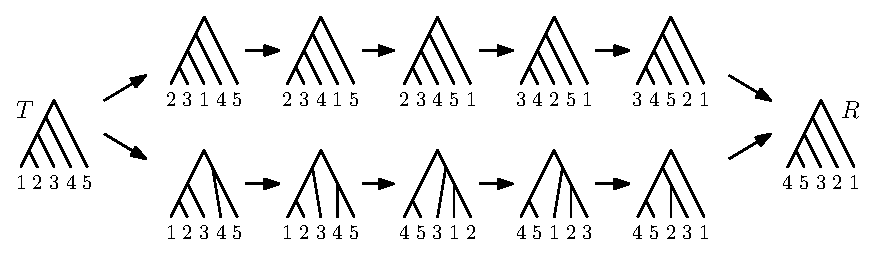
\includegraphics[width=\textwidth]{splitthm_counterexample}
    \vspace{12pt}
	\caption{The split $123|45$ is present in $T$ and $R$, but the path at the top is a shortest path (computed by $\csort$) where none of the trees contains this split.
    However, this split is maintained on the path at the bottom, which is a shortest path as well.}
	\label{fig:splitthm_counterexample}
\end{figure}

Since the counterexample in Figure~\ref{fig:splitthm_counterexample} shows that the version of the Split Theorem stated in \autocite{Gavryushkin2018-ol} does not hold, we will now claim an alternative to this conjecture, the \emph{Cluster Theorem} (Conjecture~\ref{conjecture:cluster_theorem}).
Within the Cluster Theorem we are considering clusters instead of splits.
This is motivated by the fact that rooted phylogenetic trees can uniquely be represented by sets of clusters \autocite{Steel2016-ye}, but not by sets of splits as they cannot define the position of the root.
Moreover, a ranked tree can be uniquely determined by ordering the clusters such that the ranks of the internal nodes inducing those clusters increase.
We already used this representation of trees for the algorithms in Section~\ref{section:algorithms}.

\begin{conjecture}[Cluster Theorem]
	For the $\rnni$ graph the following statement holds:
	if two trees $T$ and $R$ contain the same cluster $C$, then $C$ is present as cluster in every tree on every shortest path between $T$ and $R$.
	\label{conjecture:cluster_theorem}
\end{conjecture}

Note that trees $T$ and $R$ in Figure~\ref{fig:splitthm_counterexample} induce the same set of splits, but have distinct clusters.
Furthermore, this counterexample can be used to prove that the Cluster Theorem does not hold in $\nni$.

For providing further evidence that the Cluster Theorem holds in $\rnni$, we can show computationally that it holds for the $\rnni$ graph on small trees with up to seven taxa.
\todo{LC: We still need to check 7 taxa.}
We are doing this in the following way.
We focus on the subset of trees that induce share a cluster.
It is sufficient to consider clusters of the shape $\{1, \ldots, m\}$ for $2 \leq m \leq n-1$, because of the symmetry of the space:.
distances $d(T_1,R_1)$ and $d(T_2,R_2)$ between two pairs of trees $(T_1,R_1)$ and $(T_2,R_2)$ are equal if one can receive $T_2$ from $T_1$ by permuting the taxa the same way as it is necessary for receiving $R_2$ from $R_1$.
Therefore, we compute for all $m = 2, \ldots, n-1$ exact $\rnni$ distances between all pairs of trees containing the cluster $\{1, \ldots, m\}$, using Dijkstra's algorithm \autocite{Dijkstra1959-ph} on the $\rnni$ graph, which we can compute as explained in Section~\ref{section:alg_RNNI_graph}.
Additionally, we compute the subgraph of $\rnni$ induced by the subset of trees that include the cluster $\{1, \ldots, m\}$.
With the Floyd-Warshall algorithm we compute all pairwise distances between the trees in this subgraph and compare them with the distances in $\rnni$.
With this approach it is possible to show that the Cluster Theorem holds for up to seven taxa.
\todo{LC: We still need to check 7 taxa.}


\section{Ideas}
\todo{This section is just a rough draft. Are there ideas we want to keep? Shall this become an 'open problems/future work' section?}


The paths computed by $\findpath$ depend on the order of input trees $T$ and $R$:
$\findpath(T,R)$ does not necessarily produce the reverse path of $\findpath(R,T)$.
An example can be found in Figure~\ref{fig:findpath_not_symmetric}.
However, simulations suggest that the lengths of the two paths computed by $\findpath$ for one pair of trees are equal.

\begin{conjecture}
    Let $T$ and $R$ be ranked trees.
    The lengths of paths $\findpath(T,R)$ and $\findpath(R,T)$ are equal.
\end{conjecture}

\begin{figure}[H]
	\centering
	\includegraphics[width=0.7\textwidth]{findpath_not_symmetric}
    \vspace{12pt}
	\caption{Two paths computed by $\findpath$. At the top $\findpath(T,R)$, at the bottom $\findpath(R,T)$}
	\label{fig:findpath_not_symmetric}
\end{figure}

% idea for description of max distance caterpillar trees:
\begin{lemma}
    Let $T$ and $R$ be caterpillar trees.
    It is $d_c(T,R) = \Delta(\rnni)$ if, and only if, $T$ and $R$ share no induced triplet.
    \todo{define induced triplets}
\end{lemma}

This Lemma does only hold for caterpillar trees and not for trees with more than one cherry.
Furthermore, triplets do not represent ranked trees uniquely as they do not contain information about the ranks of internal nodes (but they can uniquely define caterpillar trees as these only have one cherry)

\begin{proof}
    %TODO
    % Insert the proof here
    Fix $T = (\ldots(1,2) \ldots ,n)$, use induction on $n$ and $\csort$ (taxon $n$ must be in cherry of $R$ if distance is max).
\end{proof}

According to Algorithm~\ref{alg:max_dist_tree}, the number of trees with maximum distance to a given caterpillar tree $T$ is $(n-1)!$.
The number of caterpillar trees with distance $\Delta(\rnni)$ from a given caterpillar tree is $2^{n-2}$.


\subsection{Partition lattice}

% Define Partition Lattice $\Pi_n$ and max chains in that lattice!

\begin{theorem}
The $\rnni$ graph on $n$ taxa is isomorphic to the graph of maximal chains of the partition lattice $\Pi_n$ where two maximal chains are connected by an edge if and only if they differ by exactly one partition.
The corresponding metric spaces are isometric.
\end{theorem}


\printbibliography

\end{document}
